\documentclass[twoside,11pt,a4paper]{article}

\usepackage[utf8]{inputenc}
\usepackage{amsmath, amssymb, latexsym}

\usepackage[left=2cm,right=2cm,top=2cm,bottom=2cm]{geometry}
\usepackage{tikz}
\usetikzlibrary{decorations.pathreplacing}
\usetikzlibrary{fadings}


\definecolor{lightblue}{rgb}{0.65,0.78,0.92}
\definecolor{lightgreen}{rgb}{0.62,0.88,0.58}
\definecolor{lightpurple}{rgb}{0.87,0.61,.93}
\definecolor{lightorange}{rgb}{0.95,0.82,0.58}
\definecolor{lightgray}{rgb}{0.8,0.8,0.8}


% args = position, width, height, depth, color, top label, bottom label
\newcommand{\drawcnnlayer}[7]{
  \path (0,0);
  \begin{scope}[shift={#1}]
  \draw[black,fill=#5] (0,0,0) -- ++(-#2,0,0) -- ++(0,-#3,0) -- ++(#2,0,0) -- cycle;
  \draw[black,fill=#5] (0,0,0) -- ++(0,0,-#4) -- ++(0,-#3,0) -- ++(0,0,#4) -- cycle;
  \draw[black,fill=#5] (0,0,0) -- ++(-#2,0,0) -- ++(0,0,-#4) -- ++(#2,0,0) -- cycle;
  %% \node at (0,#4) {#6};
  %% \node at (0,-#4) {#7};
  \end{scope}
  }


\begin{document}



\begin{figure}
  \begin{center}
    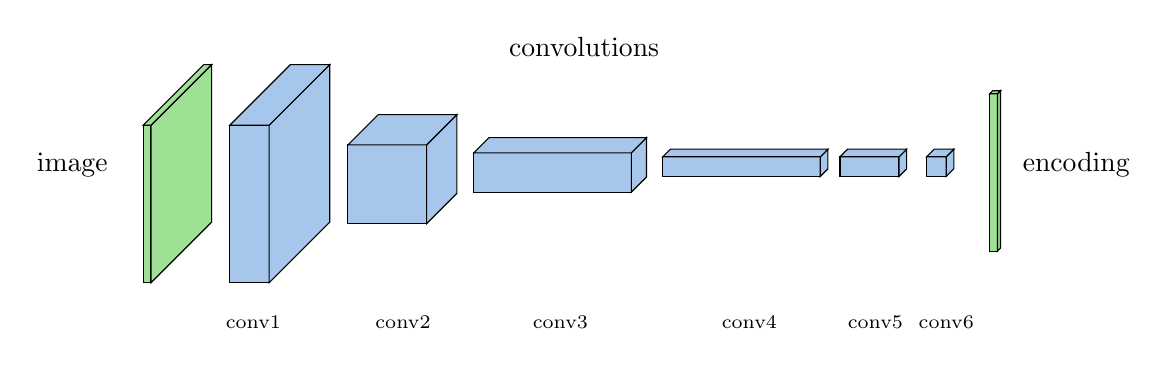
\begin{tikzpicture}
      \node at (-1,-.5) {image};
      \drawcnnlayer{(0,0)}{0.1}{2}{2}{lightgreen}{image}{};
      \node at (5.5,1) {convolutions};
      \node at (1.3,-2.5) {\scriptsize{conv1}};
      \drawcnnlayer{(1.5,0)}{0.5}{2}{2}{lightblue}{conv1}{5:2\#64};
      \node at (3.2,-2.5) {\scriptsize{conv2}};
      \drawcnnlayer{(3.5,-0.25)}{1.0}{1}{1}{lightblue}{conv2}{5:2\#128};
      \node at (5.2,-2.5) {\scriptsize{conv3}};
      \drawcnnlayer{(6.1,-0.35)}{2.0}{0.5}{0.5}{lightblue}{conv3}{5:2\#256};
      \node at (7.6,-2.5) {\scriptsize{conv4}};
      \drawcnnlayer{(8.5,-0.4)}{2.0}{.25}{.25}{lightblue}{conv4}{5:2\#256};
      \node at (9.2,-2.5) {\scriptsize{conv5}};
      \drawcnnlayer{(9.5,-0.4)}{0.75}{0.25}{0.25}{lightblue}{conv5}{32x32:1\#96};
      \node at (10.1,-2.5) {\scriptsize{conv6}};
      \drawcnnlayer{(10.1,-0.4)}{0.25}{0.25}{0.25}{lightblue}{conv6}{32x32:1\#32};
      \drawcnnlayer{(10.75,0.4)}{0.1}{2}{0.1}{lightgreen}{logits}{};
      \node at (11.75,-.5) {encoding};
    \end{tikzpicture}

    \vspace{1em}


    \begin{tabular}{l||l|l|l}
      layer & filter size & stride & \# filters \\
      \hline
      conv1 & 5 & 2 & 64 \\
      conv2 & 5 & 2 & 128 \\
      conv3 & 5 & 2 & 256 \\
      conv4 & 5 & 2 & 256 \\
      \hline
      conv5 & 32 & 1 & 96 \\
      conv6 & 32 & 1 & 32
    \end{tabular}

    \caption{VAE \textbf{encoder} architecture. All layers use Leaky ReLU activations. The final convolution output is flattened and represents our encoded image.}
  \end{center}
\end{figure}

\begin{figure}
  \begin{center}
    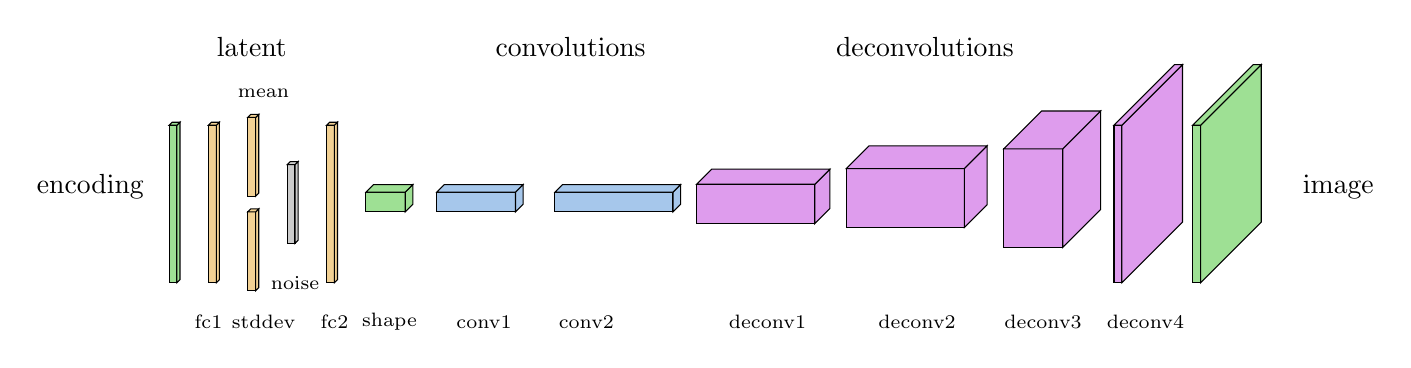
\begin{tikzpicture}
      \node at (-1.1,-.78) {encoding};
      %% \node at (-.1,-2.54) {\scriptsize{n}};
      \drawcnnlayer{(0,0)}{0.1}{2}{0.1}{lightgreen}{}{};

      
      \node at (0.95,1) {latent};
      \node at (0.40,-2.5) {\scriptsize{fc1}};
      \drawcnnlayer{(0.5,0)}{0.1}{2}{0.1}{lightorange}{}{};

      \node at (1.1,.4) {\scriptsize{mean}};
      \drawcnnlayer{(1,.1)}{0.1}{1}{0.1}{lightorange}{}{};

      \node at (1.1,-2.5) {\scriptsize{stddev}};
      \drawcnnlayer{(1,-1.1)}{0.1}{1}{0.1}{lightorange}{}{};
      
      \node at (1.5,-2) {\scriptsize{noise}};
      \drawcnnlayer{(1.5,-.5)}{0.1}{1}{0.1}{lightgray}{}{};      

      \node at (2,-2.5) {\scriptsize{fc2}};
      \drawcnnlayer{(2.0,0)}{0.1}{2}{0.1}{lightorange}{}{};      
      
      \node at (2.7,-2.5) {\scriptsize{shape}};            
      \drawcnnlayer{(2.9,-0.85)}{0.5}{0.25}{0.25}{lightgreen}{}{};
      
      
      \node at (5,1) {convolutions};
      \node at (3.9,-2.5) {\scriptsize{conv1}};
      \drawcnnlayer{(4.3,-0.85)}{1}{0.25}{0.25}{lightblue}{}{};
      \node at (5.2,-2.5) {\scriptsize{conv2}};      
      \drawcnnlayer{(6.3,-0.85)}{1.5}{0.25}{0.25}{lightblue}{}{};

      \node at (9.5,1) {deconvolutions};
      \node at (7.5,-2.5) {\scriptsize{deconv1}};
      \drawcnnlayer{(8.1,-0.75)}{1.5}{0.5}{0.5}{lightpurple}{}{};
      
      \node at (9.4,-2.5) {\scriptsize{deconv2}};      
      \drawcnnlayer{(10.0,-0.55)}{1.5}{.75}{.75}{lightpurple}{}{};
      \node at (11,-2.5) {\scriptsize{deconv3}};      
      \drawcnnlayer{(11.25,-0.3)}{0.75}{1.25}{1.25}{lightpurple}{}{};
      \node at (12.3,-2.5) {\scriptsize{deconv4}};
      \drawcnnlayer{(12,0)}{0.1}{2}{2}{lightpurple}{}{};

      \drawcnnlayer{(13,0)}{0.1}{2}{2}{lightgreen}{}{};
      \node at (14.75,-.78) {image};
    \end{tikzpicture}

    \vspace{1em}


    \begin{tabular}{l||l|l|l}
      layer & filter size & stride & \# filters (or size) \\
      \hline
      fc1 & & & 512 \\
      stddev & & & 200 \\
      mean & & & 200 \\
      noise & & & 200 \\
      fc2 & & & 512 \\
      shape & & & 4x4x32\\
      \hline
      conv1 & 1 & 1 & 96 \\
      conv2 & 1 & 1 & 256 \\
      \hline
      deconv1 & 5 & 2 & 256 \\
      deconv2 & 5 & 2 & 128 \\
      deconv3 & 5 & 2 & 64 \\            
      deconv4 & 5 & 2 & 3 \\     
      
    \end{tabular}

    
  \end{center}
  \caption{VAE \textbf{decoder} architecture. The latent is generated by remapping the encoding into two vectors representing the \emph{mean} and the \emph{standard deviation} of a Gaussian, which is then (via the reparameterization trick) used to generate a Gaussian. This is then mapped back out through a dense layer before reshaping into a small, but deep, image. This is then run through two convolution filters to expand the number of filters before upscaling with deconvolution operations.}
\end{figure}





\begin{figure}
  \begin{center}
    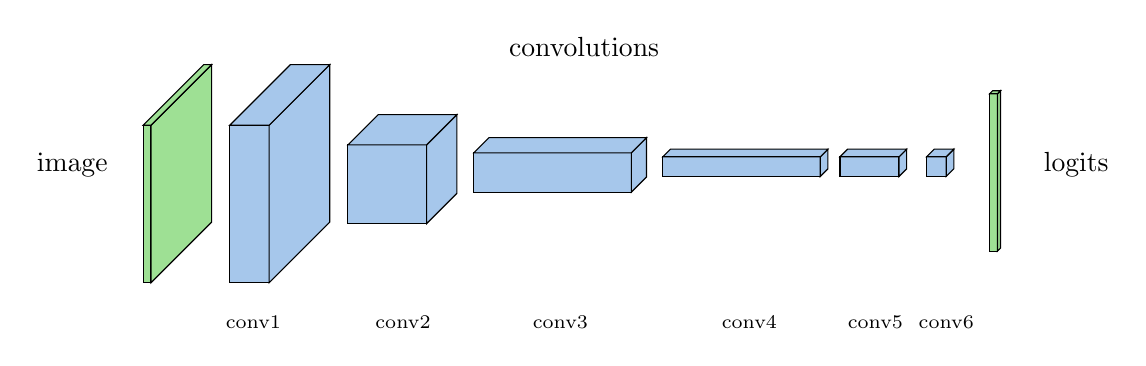
\begin{tikzpicture}
      \node at (-1,-.5) {image};
      \drawcnnlayer{(0,0)}{0.1}{2}{2}{lightgreen}{image}{};
      \node at (5.5,1) {convolutions};
      \node at (1.3,-2.5) {\scriptsize{conv1}};
      \drawcnnlayer{(1.5,0)}{0.5}{2}{2}{lightblue}{conv1}{5:2\#64};
      \node at (3.2,-2.5) {\scriptsize{conv2}};
      \drawcnnlayer{(3.5,-0.25)}{1.0}{1}{1}{lightblue}{conv2}{5:2\#128};
      \node at (5.2,-2.5) {\scriptsize{conv3}};
      \drawcnnlayer{(6.1,-0.35)}{2.0}{0.5}{0.5}{lightblue}{conv3}{5:2\#256};
      \node at (7.6,-2.5) {\scriptsize{conv4}};
      \drawcnnlayer{(8.5,-0.4)}{2.0}{.25}{.25}{lightblue}{conv4}{5:2\#256};
      \node at (9.2,-2.5) {\scriptsize{conv5}};
      \drawcnnlayer{(9.5,-0.4)}{0.75}{0.25}{0.25}{lightblue}{conv5}{32x32:1\#96};
      \node at (10.1,-2.5) {\scriptsize{conv6}};
      \drawcnnlayer{(10.1,-0.4)}{0.25}{0.25}{0.25}{lightblue}{conv6}{32x32:1\#32};
      \drawcnnlayer{(10.75,0.4)}{0.1}{2}{0.1}{lightgreen}{logits}{};
      \node at (11.75,-.5) {logits};
    \end{tikzpicture}

    \vspace{1em}


    \begin{tabular}{l||l|l|l}
      layer & filter size & stride & \# filters \\
      \hline
      conv1 & 5 & 2 & 64 \\
      conv2 & 5 & 2 & 128 \\
      conv3 & 5 & 2 & 256 \\
      conv4 & 5 & 2 & 256 \\
      \hline
      conv5 & 32 & 1 & 96 \\
      conv6 & 32 & 1 & 32
    \end{tabular}
  \end{center}

  \caption{GAN/WGAN \textbf{discriminator} architecture. In the original GAN/WGAN architecture, all convolution layers use batch normalization and a leaky ReLU activation function. In the improved WGAN architecture, batch norm is omitted. All three models use \emph{sigmoid} activation in the logits layer.}
\end{figure}



\begin{figure}
  \begin{center}
    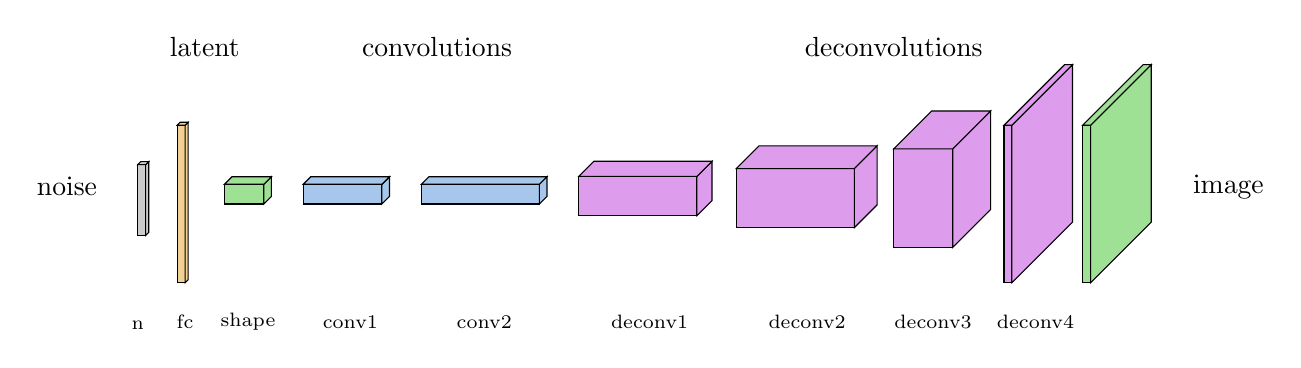
\begin{tikzpicture}
      \node at (-1,-.78) {noise};
      \node at (-.1,-2.54) {\scriptsize{n}};      
      \drawcnnlayer{(0,-.5)}{0.1}{.9}{0.1}{lightgray}{}{};
      \node at (0.75,1) {latent};
      \node at (0.50,-2.5) {\scriptsize{fc}};      
      \drawcnnlayer{(0.5,0)}{0.1}{2}{0.1}{lightorange}{}{};
      \node at (1.3,-2.5) {\scriptsize{shape}};            
      \drawcnnlayer{(1.5,-0.75)}{0.5}{0.25}{0.25}{lightgreen}{}{};
      
      
      \node at (3.7,1) {convolutions};
      \node at (2.6,-2.5) {\scriptsize{conv1}};
      \drawcnnlayer{(3.0,-0.75)}{1}{0.25}{0.25}{lightblue}{}{};
      \node at (4.3,-2.5) {\scriptsize{conv2}};      
      \drawcnnlayer{(5.0,-0.75)}{1.5}{0.25}{0.25}{lightblue}{}{};

      \node at (9.5,1) {deconvolutions};
      \node at (6.4,-2.5) {\scriptsize{deconv1}};
      \drawcnnlayer{(7.0,-0.65)}{1.5}{0.5}{0.5}{lightpurple}{}{};
      \node at (8.4,-2.5) {\scriptsize{deconv2}};      
      \drawcnnlayer{(9.0,-0.55)}{1.5}{.75}{.75}{lightpurple}{}{};
      \node at (10,-2.5) {\scriptsize{deconv3}};      
      \drawcnnlayer{(10.25,-0.3)}{0.75}{1.25}{1.25}{lightpurple}{}{};
      \node at (11.3,-2.5) {\scriptsize{deconv4}};
      \drawcnnlayer{(11,0)}{0.1}{2}{2}{lightpurple}{}{};

      \drawcnnlayer{(12,0)}{0.1}{2}{2}{lightgreen}{}{};
      \node at (13.75,-.78) {image};
    \end{tikzpicture}

    \vspace{1em}


    \begin{tabular}{l||l|l|l}
      layer & filter size & stride & \# filters (or size) \\
      \hline
      n & & & 200 \\
      fc & & & 512 \\
      shape & & & 4x4x32 \\
      \hline
      conv1 & 1 & 1 & 96 \\
      conv2 & 1 & 1 & 256 \\
      \hline
      deconv1 & 5 & 2 & 256 \\
      deconv2 & 5 & 2 & 128 \\
      deconv3 & 5 & 2 & 64 \\            
      deconv4 & 5 & 2 & 3 \\     
      
    \end{tabular}

    
  \end{center}
  \caption{GAN/WGAN \textbf{generator} architecture. Starting with a latent vector of Gaussian noise, we expand it using a fully connected layer and then reshape it into an image with depth. The number of filters is then expanded further using convolutions before upscaling it several times using deconvolution operations. Each (de)convolution layer uses batch normalization and a ReLU activation function, and the final output values are rescaled with \emph{tanh}.}
\end{figure}



\end{document}
